\documentclass[14pt,a4paper]{book}

% Използване на български език.
\usepackage[english,bulgarian]{babel}
\usepackage[utf8]{inputenc}

% Използване на графика.
\usepackage[pdftex]{graphicx}

% Използване на PDF-и за кориците.
\usepackage{pdfpages}

% Използване на хедър и футър.
\usepackage{fancyhdr}

% Използване на кавички при цитиране.
\usepackage{dirtytalk}

% Използва се за създаване на азбучен указател.
\usepackage{imakeidx}

% Използва се за сензитивни хипер-връзки в самия документ.
\usepackage[pdftex, bookmarks, linktocpage]{hyperref}

% Използва се за листинги с програмен код.
\usepackage{listings}

% Заглавие.
\title{Блоково програмиране със Scratch и App Inventor}

% Автори.
\author{Тодор Балабанов, Галя Петрова}

% Директория с изображения.
\graphicspath{{images/}}

% Избор на активен език.
\selectlanguage{bulgarian}

% Текстове за декорация на страницата в горната и долната част.
\pagestyle{fancy}
\fancyhf{}
\fancyhead[LE,RO]{\thepage}
\fancyhead[RE]{Блоково програмиране със Scratch и App Inventor}
\fancyhead[LO]{Тодор Балабанов, Галя Петрова}
\fancyfoot[LE,RO]{Издателство \say{Образование и Познание}, 2020}

% Дебелина на разделителните линии.
\renewcommand{\headrulewidth}{2pt}
\renewcommand{\footrulewidth}{1pt}

% Генериране на азбучен указател.
\onecolumn
\makeindex[columns=2, title=Азбучен указател, intoc]

% Подменя думата използван а за ноемрация на фрагментите програмен код.
\renewcommand{\lstlistingname}{Листинг}

% Смяна на названието за списъка от листингите.
\renewcommand{\lstlistlistingname}{Списък на листингите}

% Определя характеристиките на листигните за програмния код.
\lstset{backgroundcolor=\color{gray!30}, breaklines=true, language=r, frame=single}

% Начало на документа.
\begin{document}

% Предна корица.
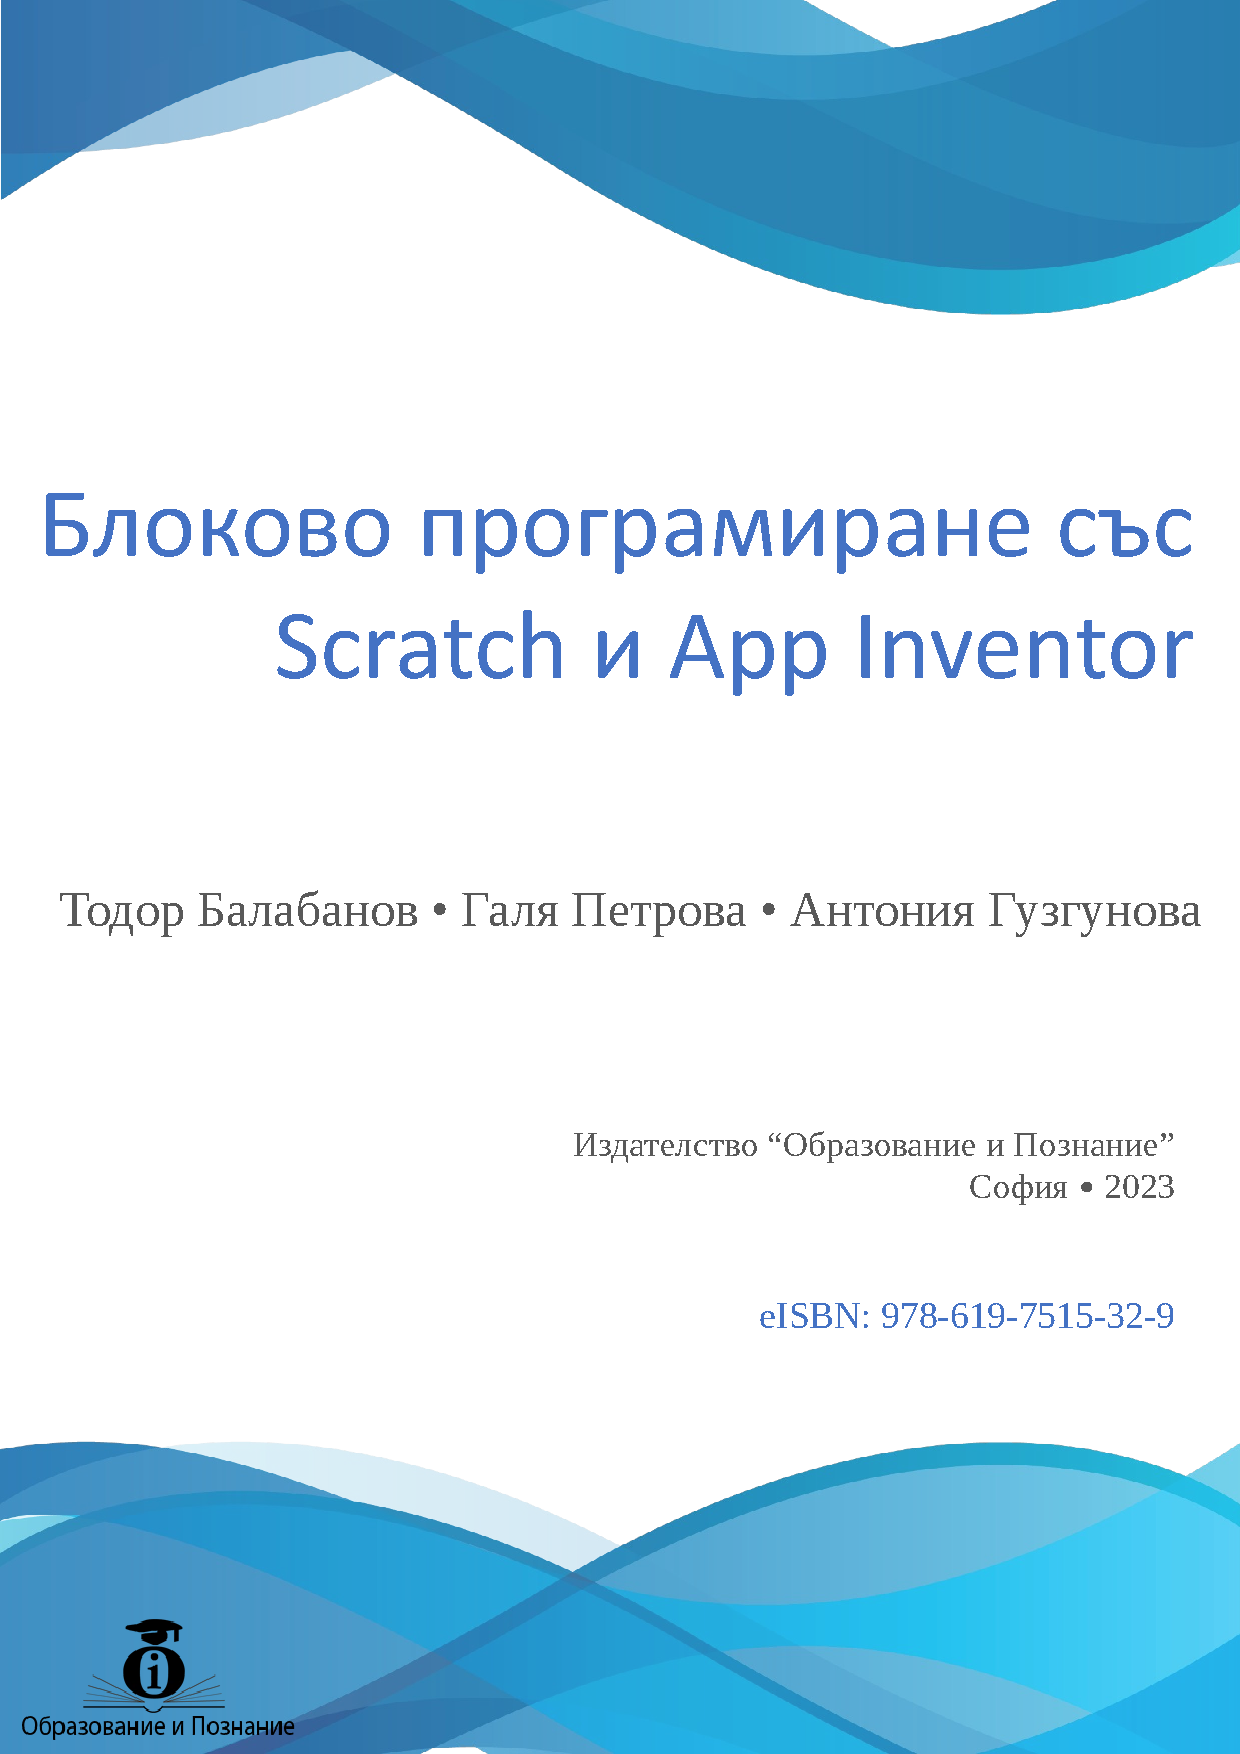
\includepdf[pages={1}]{covers/front}
\thispagestyle{empty}

% Страница с авторски права.
~\vfill
\thispagestyle{empty}

\noindent Авторски права \copyright\ 2022 \\

\noindent Тодор Балабанов, Галя Петрова \\ 

\noindent \textsc{Издателство \say{Образование и Познание}} \\
\noindent \textsc{https://www.obrazovaniebg.net/} \\

\noindent Разпространява се под свободен лиценз: \\ 
Creative Commons Attribution-NonCommercial-NoDerivatives 4.0 \\
International Public License \\
\url{https://creativecommons.org/licenses/by-nc-nd/4.0} \\

\noindent {\footnotesize This book was partially supported by the Bulgarian National Science Fund by the project \say{Mathematical models, methods and algorithms for solving hard optimization problems to achieve high security in communications and better economic sustainability, KP-06-N52/7/19-11-2021}}. \\

\noindent \textit{Първо издание, 2022}

% Номериране на страниците със служебна информация.
\pagenumbering{roman}
\setcounter{page}{1}

% Таблица на съдържанието.
\addcontentsline{toc}{chapter}{Съдържание}
\tableofcontents\newpage

% Списък с фигурите.
\addcontentsline{toc}{chapter}{Списък на фигурите}
\listoffigures\newpage

% Списък с таблиците.
\addcontentsline{toc}{chapter}{Списък на таблиците}
\listoftables\newpage

% Списък с листингите.
\addcontentsline{toc}{chapter}{Списък на листингите}
\lstlistoflistings\newpage

% Номериране на страниците с основното изложение.
\pagenumbering{arabic}
\setcounter{page}{1}

% Отделните глави са в отделни файлове.
\addcontentsline{toc}{chapter}{Предговор}
\chapter*{Предговор}
\thispagestyle{empty}

Тази книга е предназначена за всички хора, които се вълнуват от теми в програмирането и най-вече за обучението на деца в тази област. Надеждата ни е, че всеки с интерес в областта би намерил нещо ценно в изложения материал. Нашият опит е предимно свързан с академичния свят и педагогиката, посветена на обучението на деца. Материалът е изложен по такъв начин, че да разкрива основните механизми за учене чрез правене. Най-общо казано, книгата съпровожда читателя с минимални компютърни познания до едно задоволително ниво на разбиране за концепциите в програмирането. 

От наша гледна точка, представянето на програмните конструкции с помощта на визуализация, максимално доближаваща класическите пъзели, дава широки възможности за усвояване на ценни знания и умения. Подобен подход за онагледяване позволява ефективно снижаване на възрастта за обучение по програмиране. Докато класическите програмни езици са подходящи в класовете на гимназията, блоковите езици ефективно намират своето приложение в прогимназиалния курс на обучение. 

Част от изложения материал разяснява фундаментални концепции в програмирането, като - последователност от инструкции, условни и безусловни преходи, цикличност на действията, събития, модулна организация и други. Друга част набляга на практическа реализация и то на идеи, които имат потенциал да се превърнат в самостоятелни софтуерни решения. Избраният подход за представяне на информацията е чрез примери на принципа – направа, стъпка по стъпка. 

Книгата не предполага предварителни изисквания за напреднало ниво на компютърна грамотност, но разчита читателят да има базови познания за това какво е компютърна система, какво е операционна система, какво е Интернет, как се борави със зареждането и преглеждането на уеб страници. Разгледаните системи за блоково програмиране са уеб базирани и работата с тях се осъществява в облачно пространство. Не се изискват задълбочени познания по математика, но за разбирането на някои от примерите много помагат базови познания по алгебра и геометрия. Артистични умения, като музикалност или изобразителни изкуства не са нужни, но наличието им би дало допълнителен колорит на постигнатите резултати. 

Материалът е организиран в глави, които са свързани една с друга и за по-пълноценно усвояване е желателно прочитането им да се извърши в зададената последователност. Част от изложението в книгата се базира на учебни предмети, преподавани в прогимназиалния курс на обучение.

\vspace{0.5cm}

\large{\textbf{Благодарности}}

\vspace{0.5cm}

Авторите биха искали да благодарят на своите семейства за търпението и разбирането, проявено в дългият период за написването на тази книга. Също така биха искали да благодарят на своите колеги и приятели, помогнали в достигането на едно по-високо качество. 



\newpage
%\chapter{Работни среди}

Блоковите програмни езици са подразделение на визуалните програмни езици. Същината на блоковите езици е, че програмните инструкции се въвеждат под формата на цветни блокове, а не както е в класическите програмни езици, чрез изписване на текстови команди. Най-основната цел на блоковите езици е да направят областта програмиране значително по-достъпна за начинаещите. Тази цел се постига чрез три основни направления. От синтактична гледна точка, инструкциите в блоковите езици са под формата на цветни иконки. Това значително намалява възможността за изписването на грешна програмна инструкция. На второ място се подобрява семантиката, като всяка от възможните програмни инструкции е добре документирана. На трето място е прагматизма, който позволява изучаването на различните състояния в които може да изпадне програмата. Програмните среди за блоково програмиране набират все по-голяма популярност през последното десетилетие. Някои от най-популярните са: Scratch, Blockly, App Inventor for Android, Ardublock и други. В тази книга ще се спрем на две от програмните среди за блоково програмиране, създадени в Масачузетския технологичен институт, Scratch и App Inventor for Android. Причината за този избор е, че Scratch има насоченост към най-малките, а именно децата в началните училищни класове, което много добре се съчетава с възможностите блоковите програми да бъдат визуализирани и на мобилен телефон, чрез App Inventor for Android. И при двете програмни среди не се изисква инсталирането на специализиран софтуер. Достатъчно е наличието на съвременен компютър, свързан в Интернет и съвременна версия на уеб браузър. 

\section{Първи стъпки в Sratch}

Работата в средата на Sratch започва със зареждане на главната уеб страница (Фиг. \ref{fig0001}), която се намира на адрес: \\ \href{https://scratch.mit.edu/}{https://scratch.mit.edu/}

\begin{figure}[H]
  \centering
  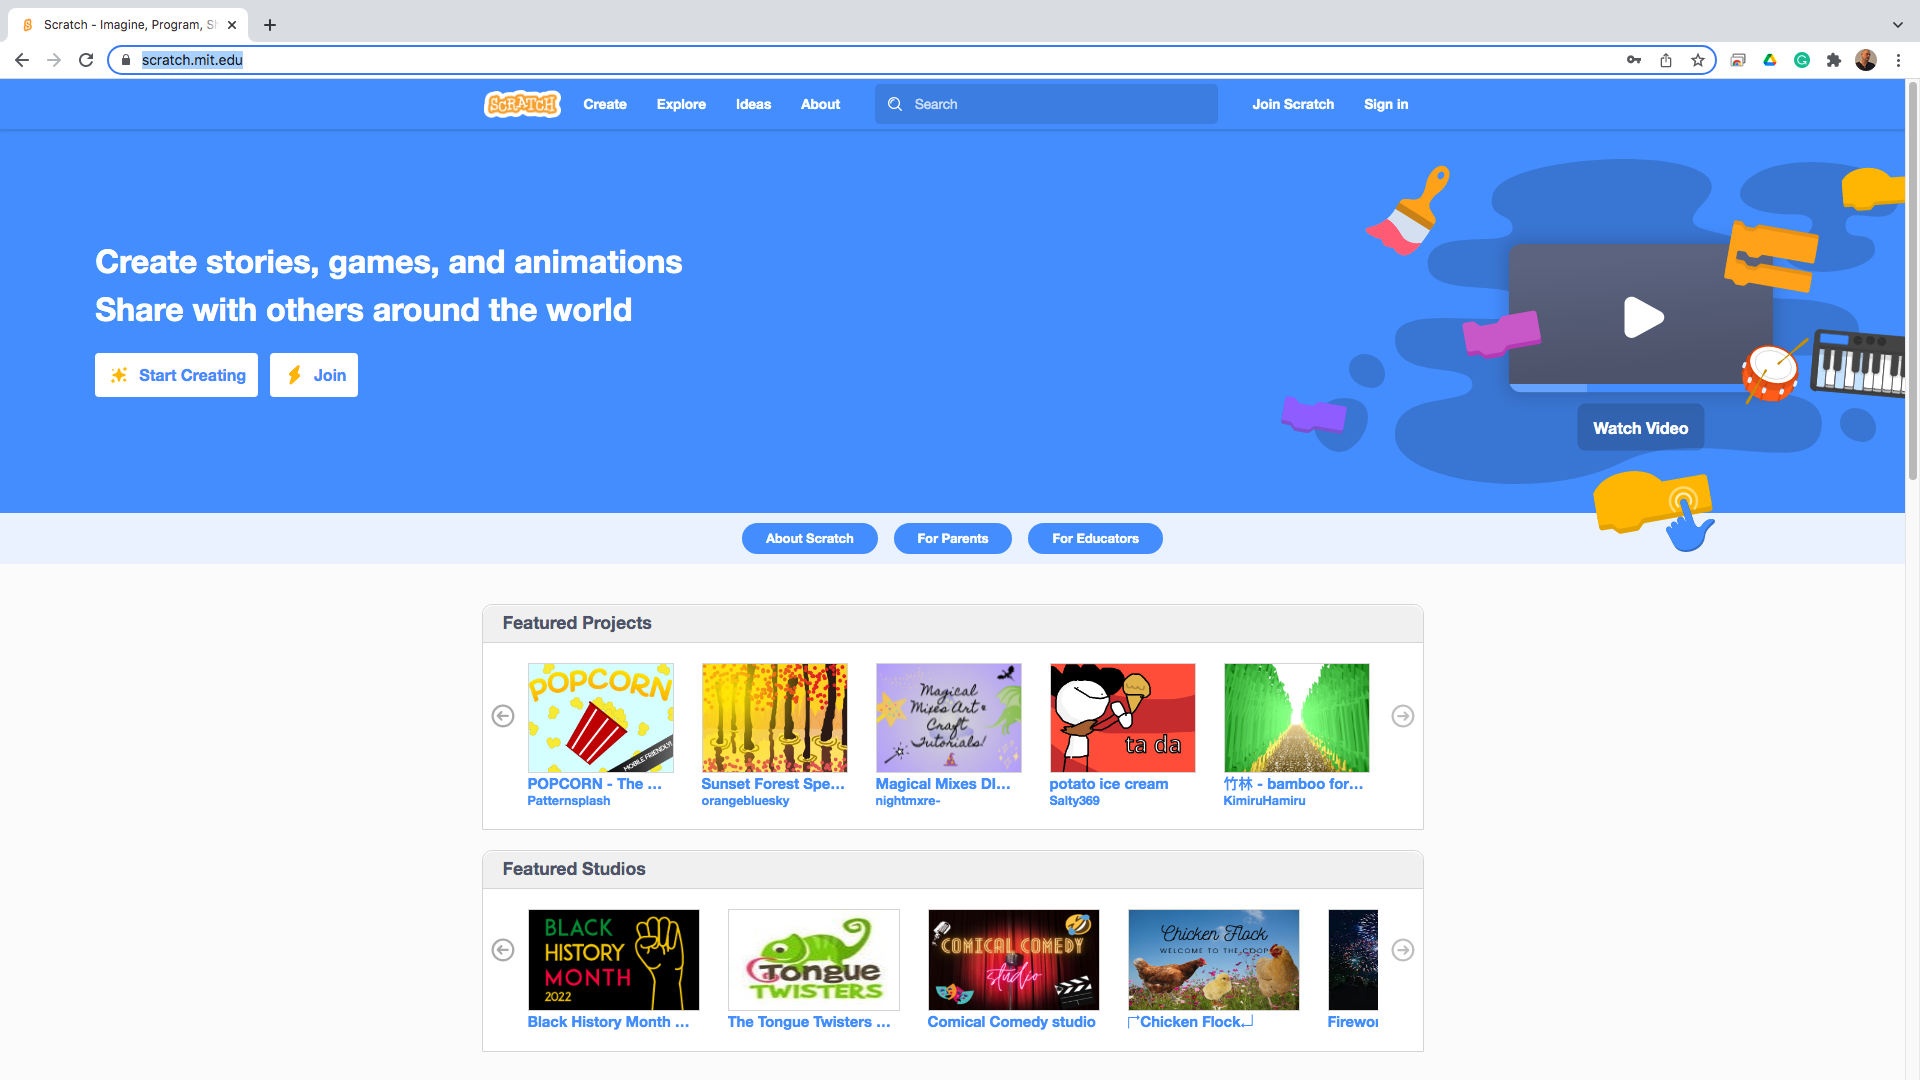
\includegraphics[width=1.0\linewidth,height=0.5\linewidth]{fig0001.png}
  \caption{Начална уеб страница на Sratch}
\label{fig0001}
\end{figure}

Програмната среда на Sratch е организирана на принципа на облачните услуги. Поради тази причина, всеки желаещ да използва услугата трябва да си направи регистрация (Фиг. \ref{fig0002}). Регистрацията се състои от потребителско име и парола.

\begin{figure}[H]
  \centering
  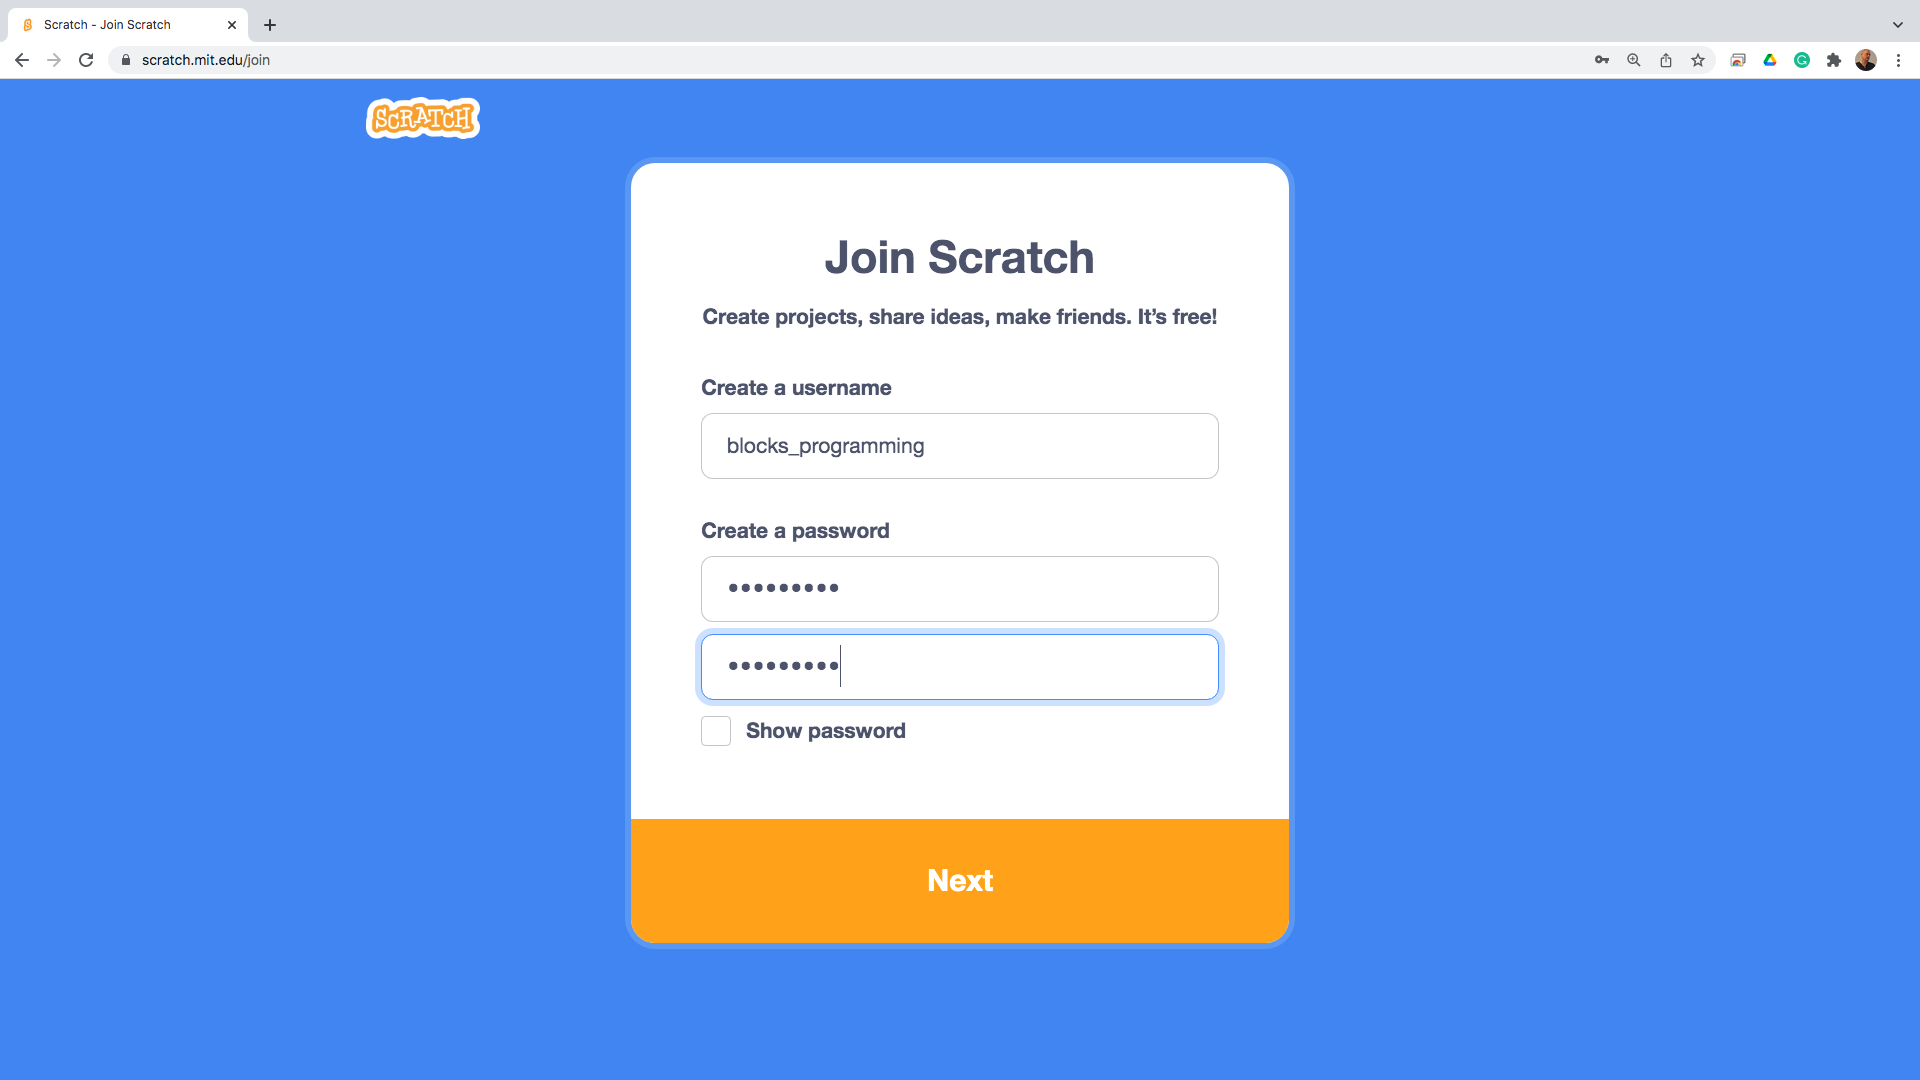
\includegraphics[width=1.0\linewidth,height=0.5\linewidth]{fig0002.png}
  \caption{Регистрация на потребител в Sratch}
\label{fig0002}
\end{figure}

След избора на потребителско име и парола следва определяне на географския регион в който се намира потребителят (Фиг. \ref{fig0003}).

\begin{figure}[H]
  \centering
  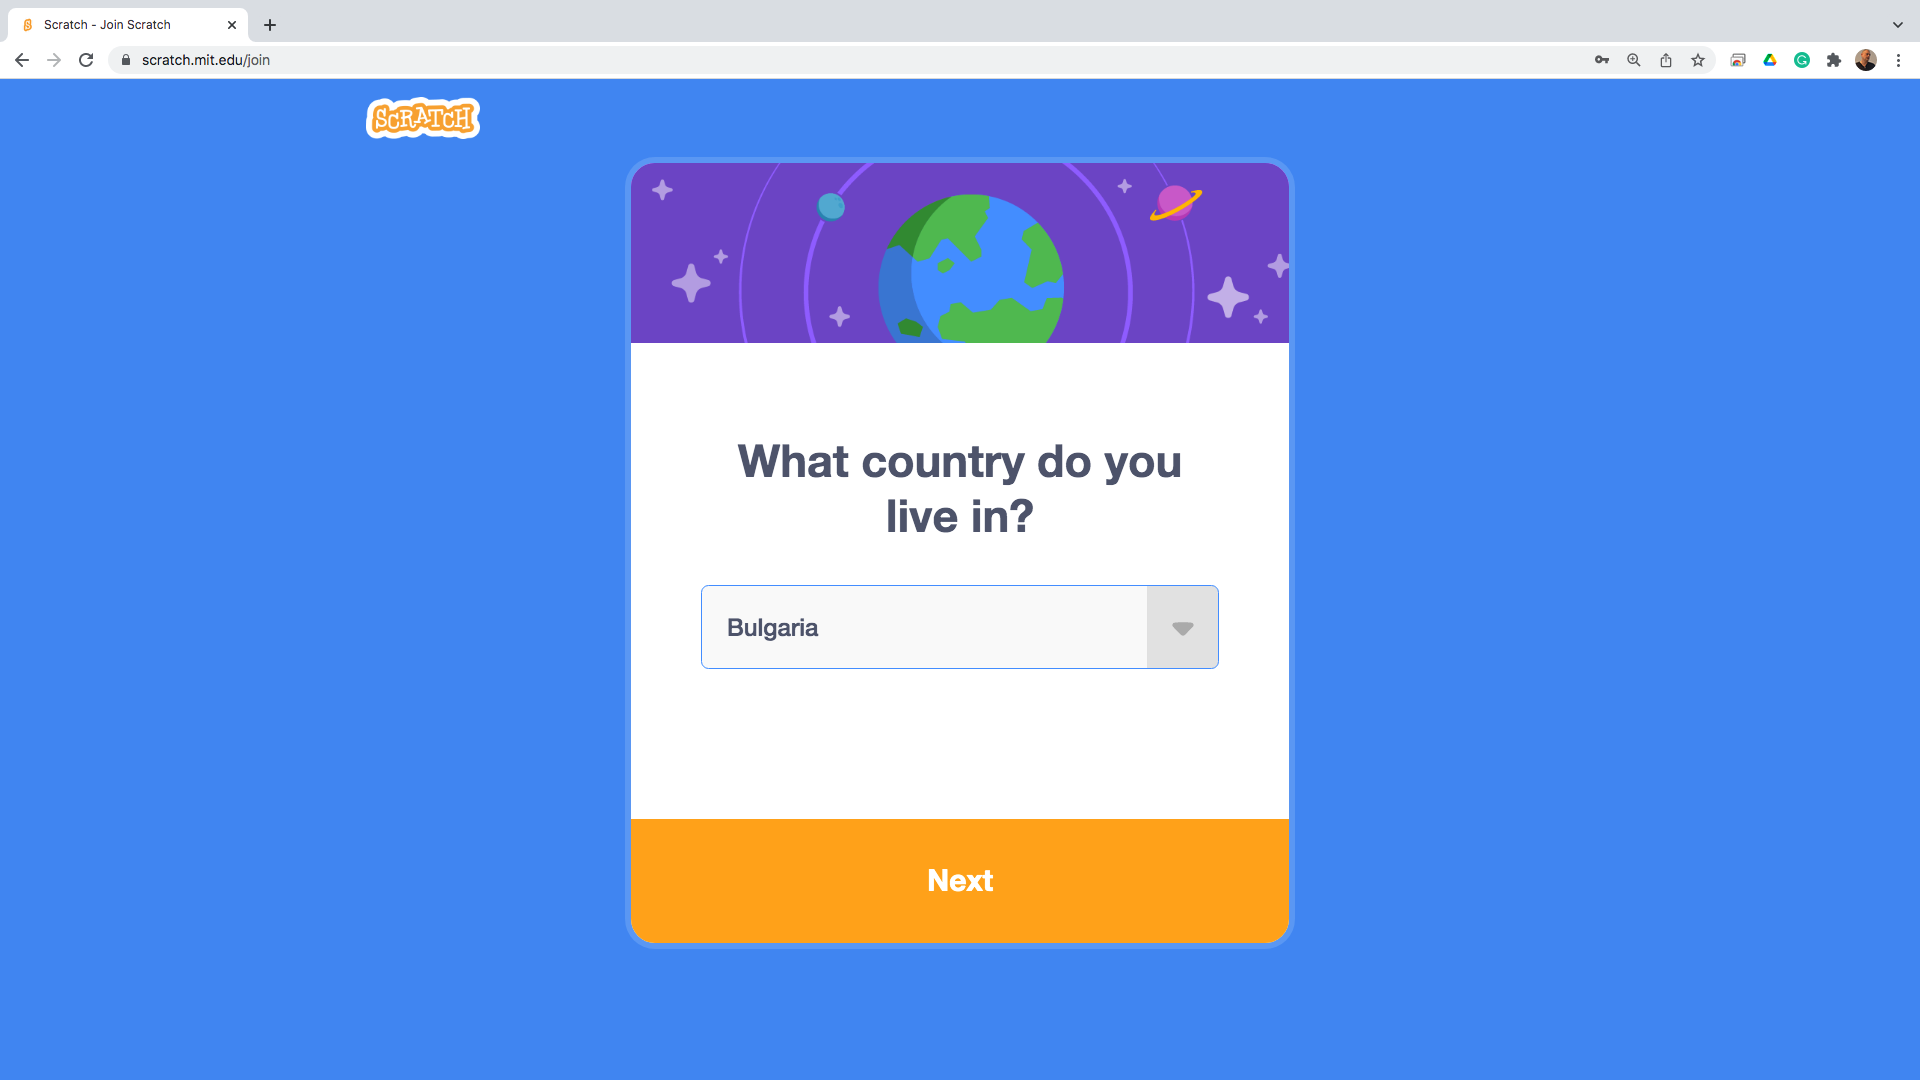
\includegraphics[width=1.0\linewidth,height=0.5\linewidth]{fig0003.png}
  \caption{Географско местоположение}
\label{fig0003}
\end{figure}

Платформата е насочена предимно към деца, изразяващи интерес към програмирането, но също така към родители и учители. Поради тази причина, системата събира информация за възрастта на потребителя (Фиг. \ref{fig0004}).

\begin{figure}[H]
  \centering
  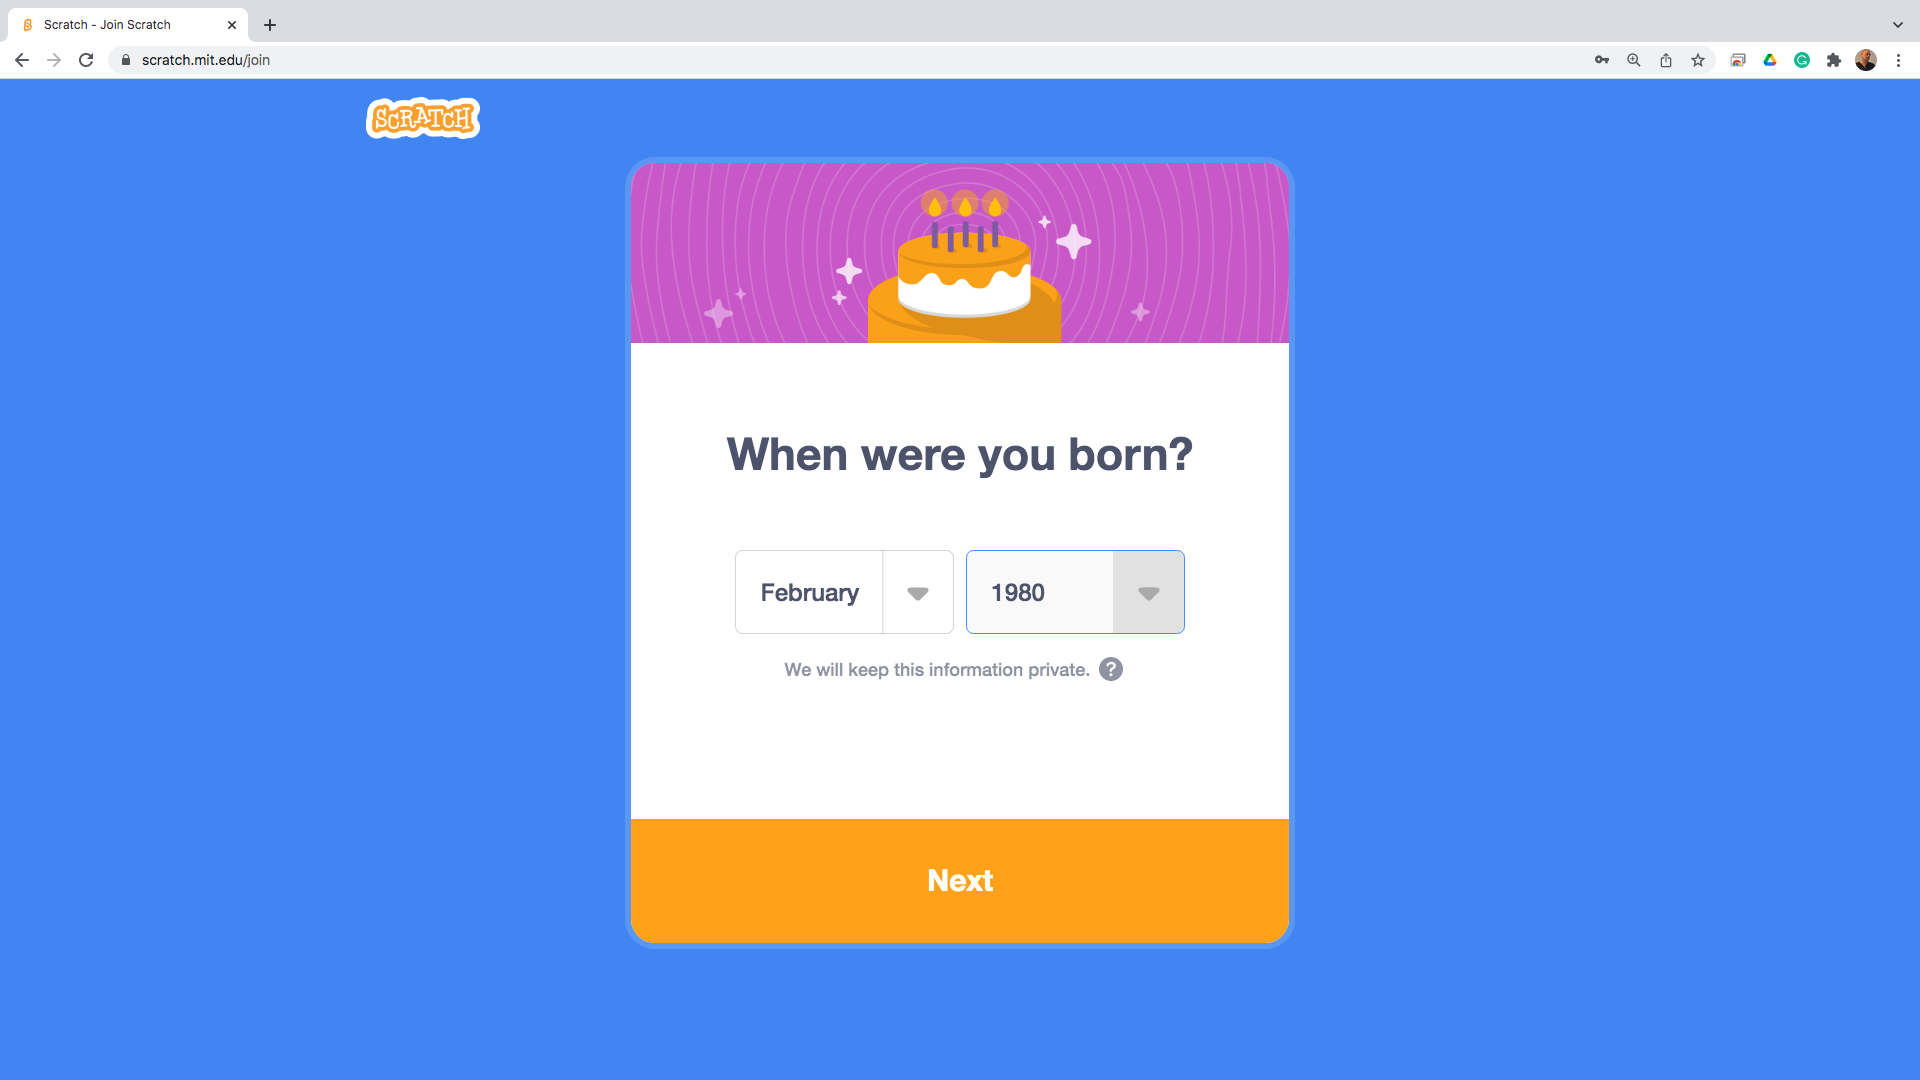
\includegraphics[width=1.0\linewidth,height=0.5\linewidth]{fig0004.png}
  \caption{Възраст на потребителя}
\label{fig0004}
\end{figure}

Освен класификация по възраст, системата събира информация и за класификация по полова принадлежност. Тази информация е незадължителна, основно за да не бъде дискриминираща (Фиг. \ref{fig0005}).

\begin{figure}[H]
  \centering
  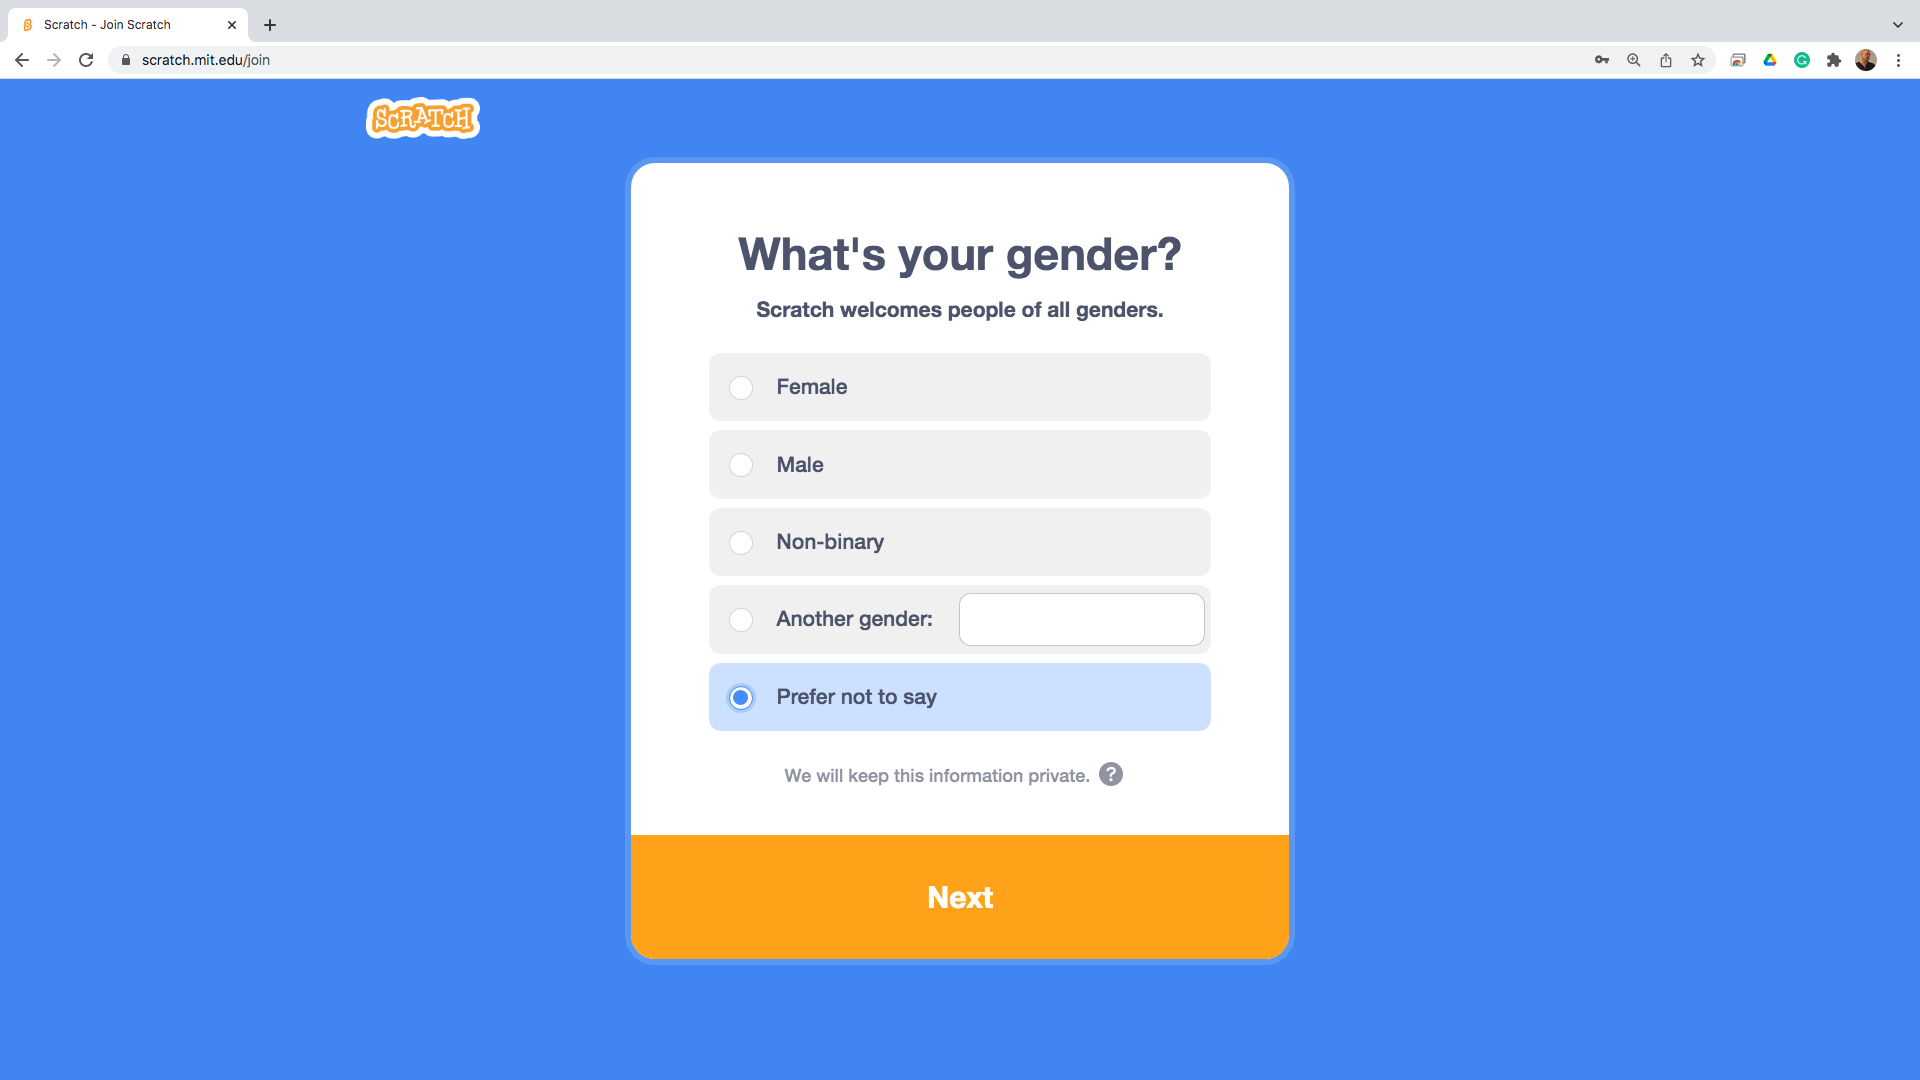
\includegraphics[width=1.0\linewidth,height=0.5\linewidth]{fig0005.png}
  \caption{Пол на потребителя}
\label{fig0005}
\end{figure}

Потребителският профил, освен с потребителско име и парола, трябва да бъде аоцииран и с адрес на електронна пощенска кутия (Фиг. \ref{fig0006}).

\begin{figure}[H]
  \centering
  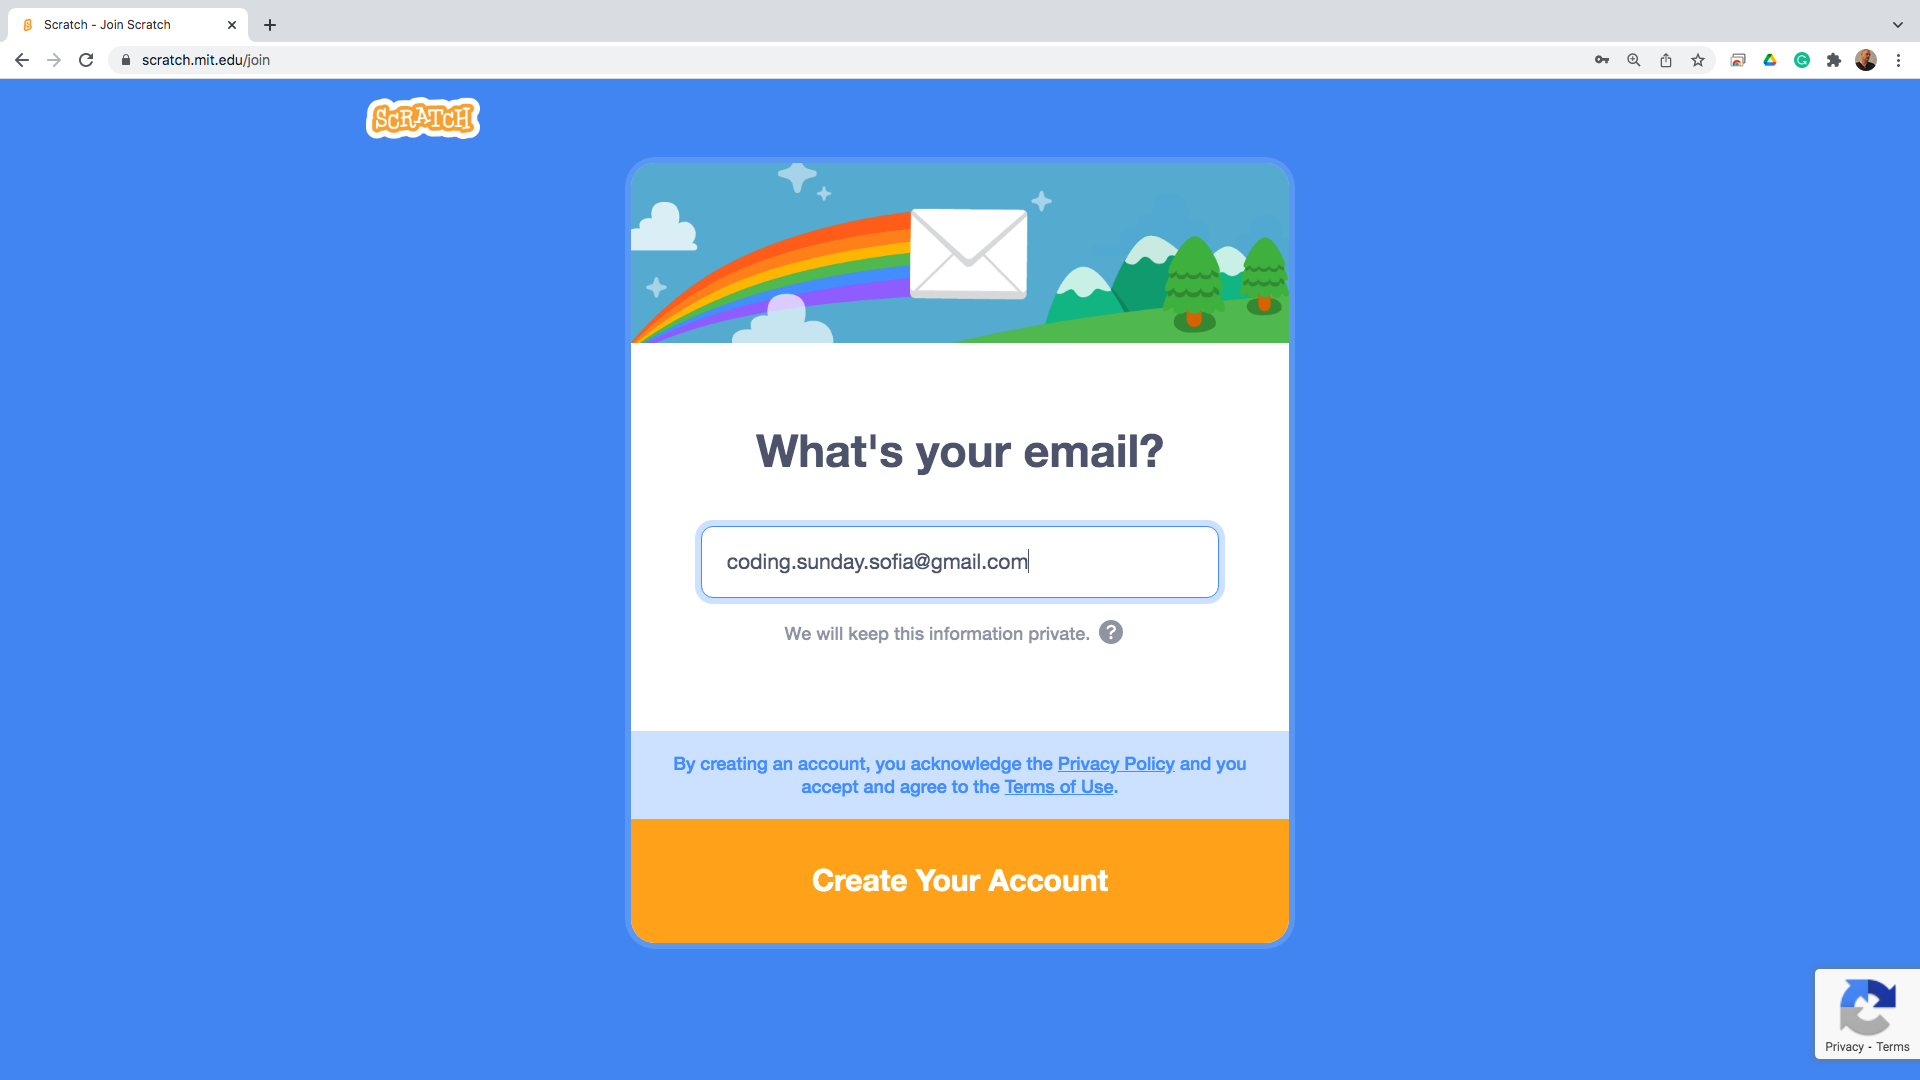
\includegraphics[width=1.0\linewidth,height=0.5\linewidth]{fig0006.png}
  \caption{Адрес на електронна поща на потребителя}
\label{fig0006}
\end{figure}

Процесът по регистрация на потребител в системата е почти завършен (Фиг. \ref{fig0007}). Остава само стъпката за потвърждаване на избрания адрес за електронна поща.

\begin{figure}[H]
  \centering
  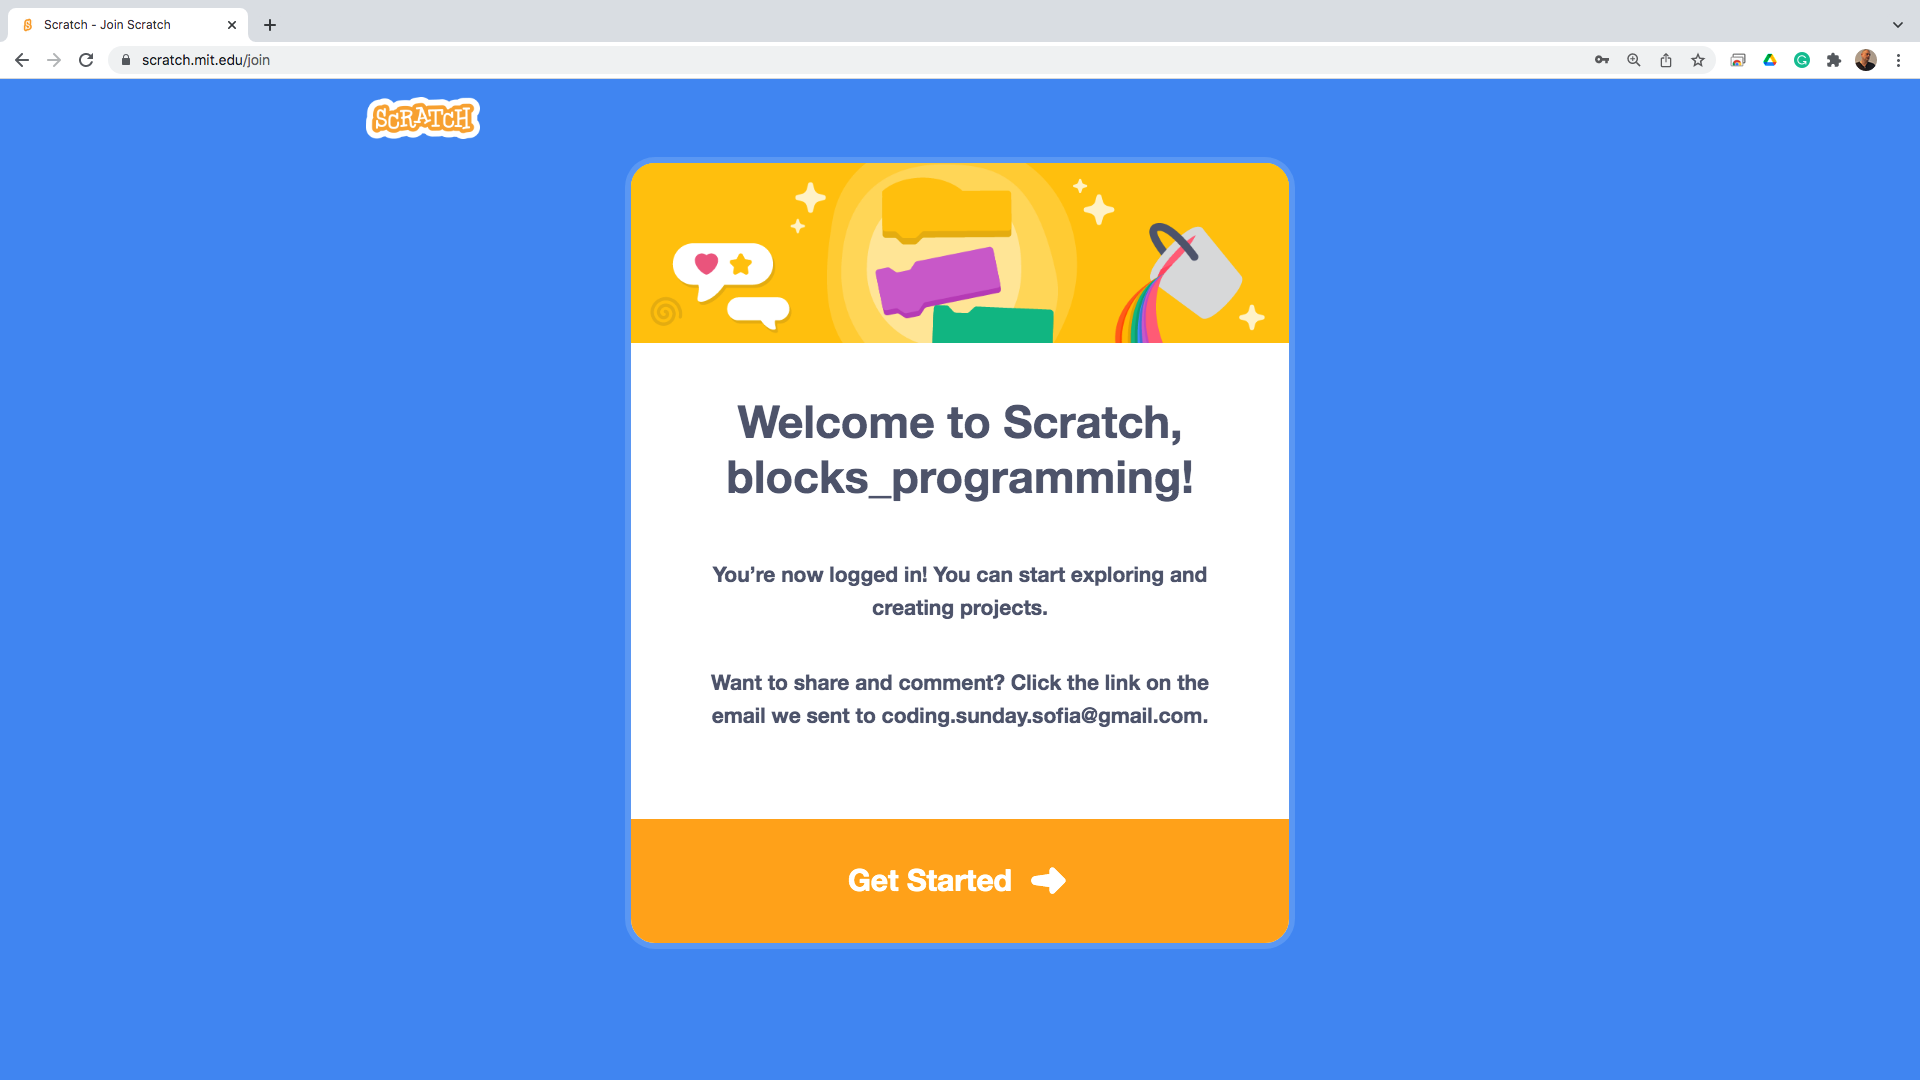
\includegraphics[width=1.0\linewidth,height=0.5\linewidth]{fig0007.png}
  \caption{Приключване на процеса за въвеждане на информация за потребителя}
\label{fig0007}
\end{figure}

Електронното писмо, за потвърждаване на потребителската регистрация, съдържа електронна препратка до уеб сайта на Sratch (Фиг. \ref{fig0008}). Тази препратка трябва да бъде последвана за да се завърши процесът по регистрация на нов потребител. 

\begin{figure}[H]
  \centering
  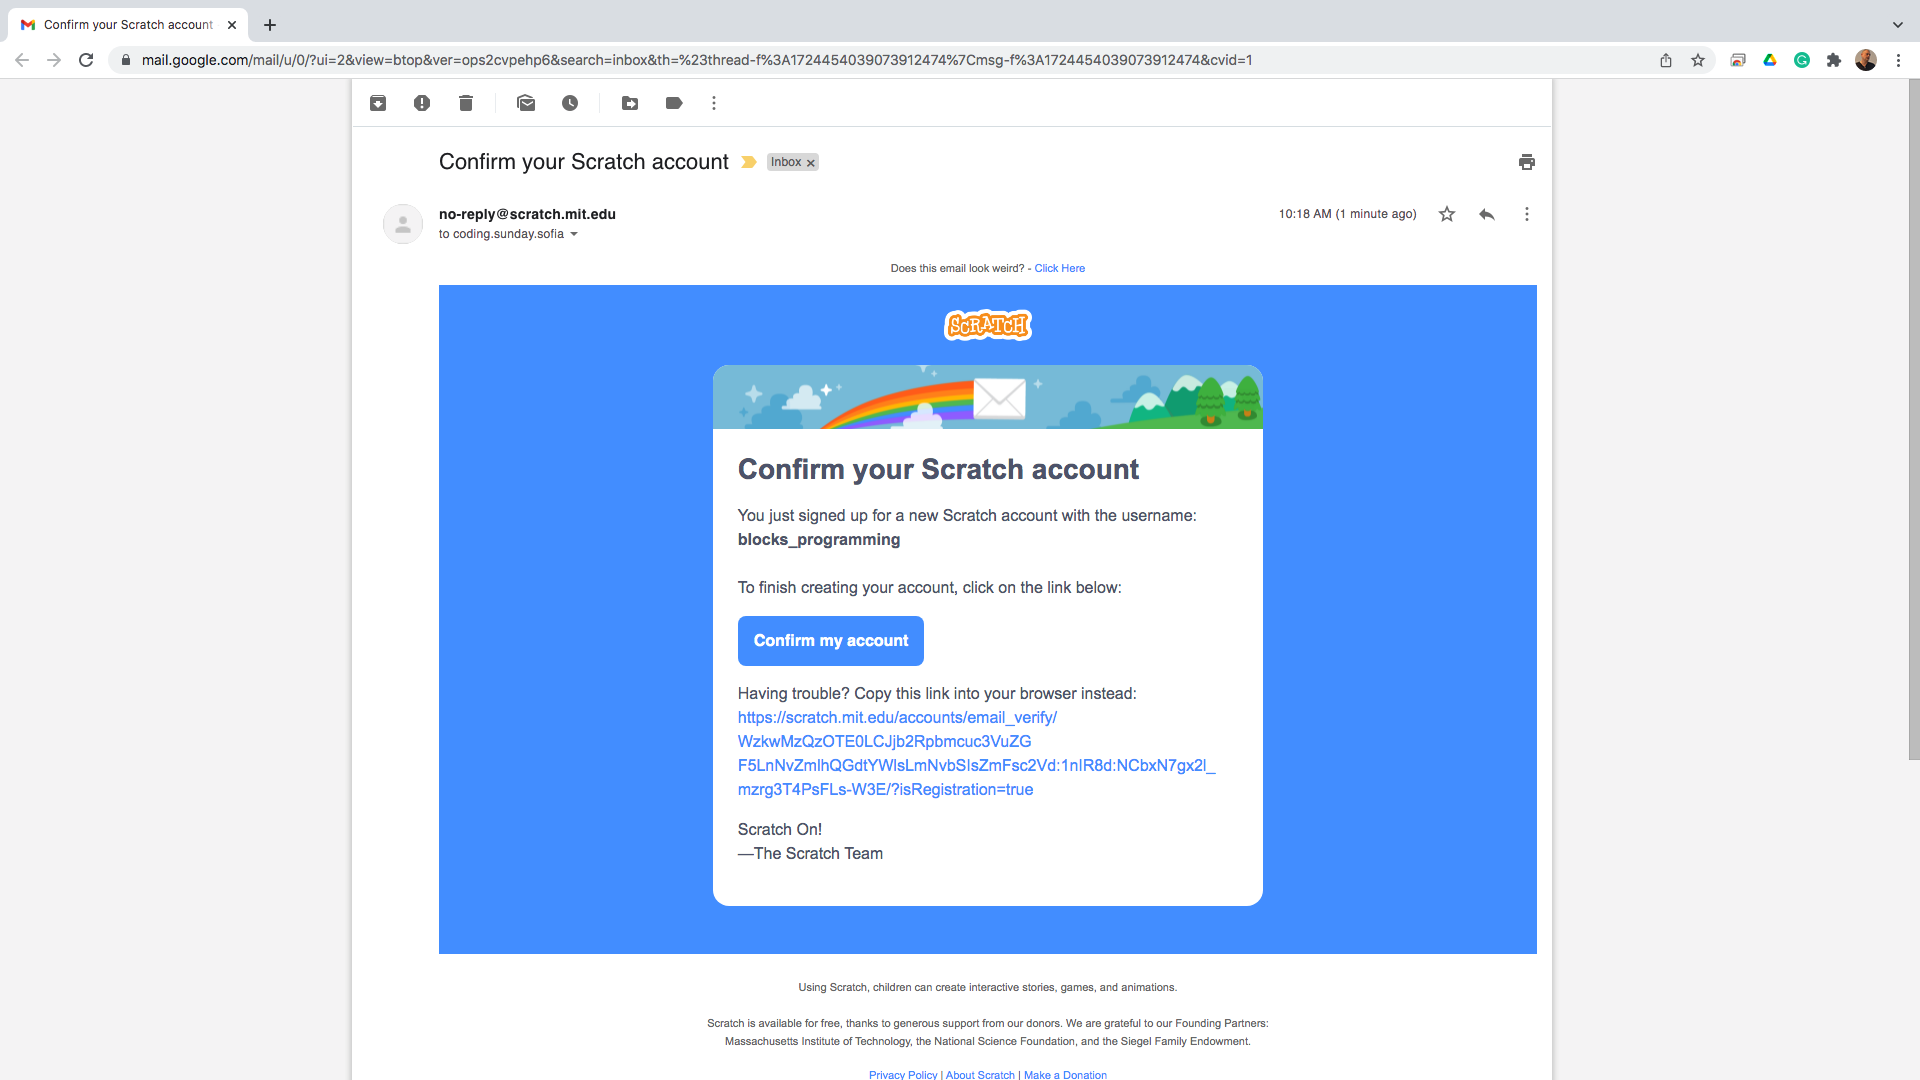
\includegraphics[width=1.0\linewidth,height=0.5\linewidth]{fig0008.png}
  \caption{Електронно съобщение за потвърждаване на електронния адрес}
\label{fig0008}
\end{figure}

Регистрацията на новия потребител приключва със зареждането на начален работен екран (Фиг. \ref{fig0009}). Горе, в дясно се вижда изписано потребителското име, избрано на първата стъпка от процеса по регистрацията.

\begin{figure}[H]
  \centering
  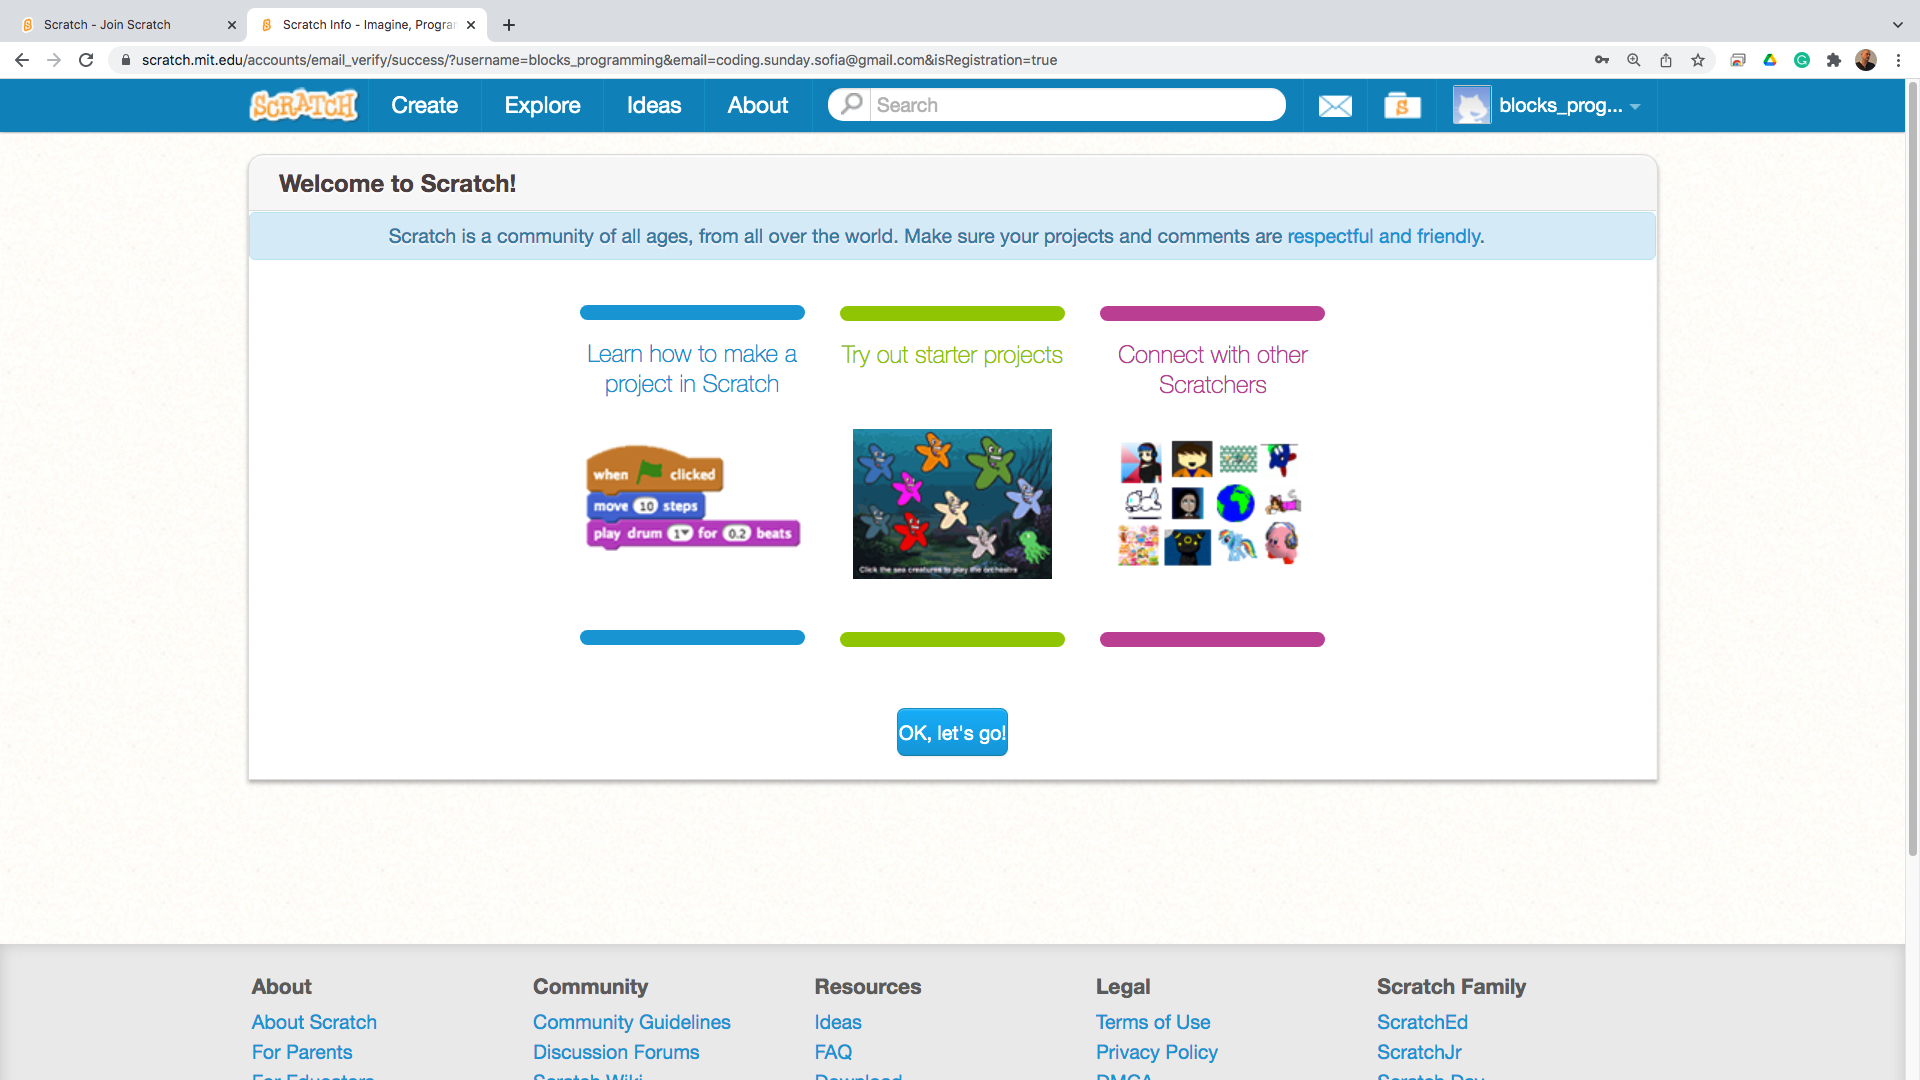
\includegraphics[width=1.0\linewidth,height=0.5\linewidth]{fig0009.png}
  \caption{Начален работен екран}
\label{fig0009}
\end{figure}

\section{Първи стъпки в App Inventor}

\newpage
\addcontentsline{toc}{chapter}{Заключение}
\chapter*{Заключение}
\thispagestyle{empty}

Блоковото програмиране е ефективен и достъпен начин за запознаване на децата с концепциите за кодиране. Чрез разбиването на програмирането на визуални блокове, децата могат да се научат да сглобяват малки програми, без да се притесняват за синтаксис или грешки при въвеждане. Програмните среди Scratch и App Inventor са доказал се в практиката инструменти за преподаване на блоково програмиране на деца. Интуитивният интерфейс и цветните блокове на Scratch го правят идеален вариант за по-малки деца, докато способността на App Inventor да създава реални мобилни приложения може да се хареса на по-големите. Книгата предоставя изчерпателно ръководство за изучаване на блоково програмиране със Scratch и App Inventor. Обхваща проектиране и създаване на игри, създаване на мобилни приложения и други. Книгата също така включва инструкции стъпка по стъпка и много визуални примери, които да помогнат на децата да разберат концепциите за програмиране. Децата могат да развият основни умения като решаване на проблеми, логическо мислене и креативност чрез блоково програмиране. Тези умения могат да бъдат приложени в бъдещи начинания, включително компютърни науки и други области от науката, технологиите, инженерството и математиката. Като цяло, книгата за блоково програмиране за деца със Scratch и App Inventor е отличен ресурс за родители и преподаватели, които искат да запознаят децата с възможностите на програмирането. Използвайки визуални блокове и лесни за разбиране инструкции, децата могат да се научат да кодират по забавен и увлекателен начин, което ги подготвя за бъдещ успех в личен и професионален план.

\newpage

% Списък с използвана литература и източници на информация.
\addcontentsline{toc}{chapter}{Библиография}
\begin{thebibliography}{99}
\end{thebibliography}
\newpage

% Азбучен указател на използваните термини.
\printindex

% Задна корица.
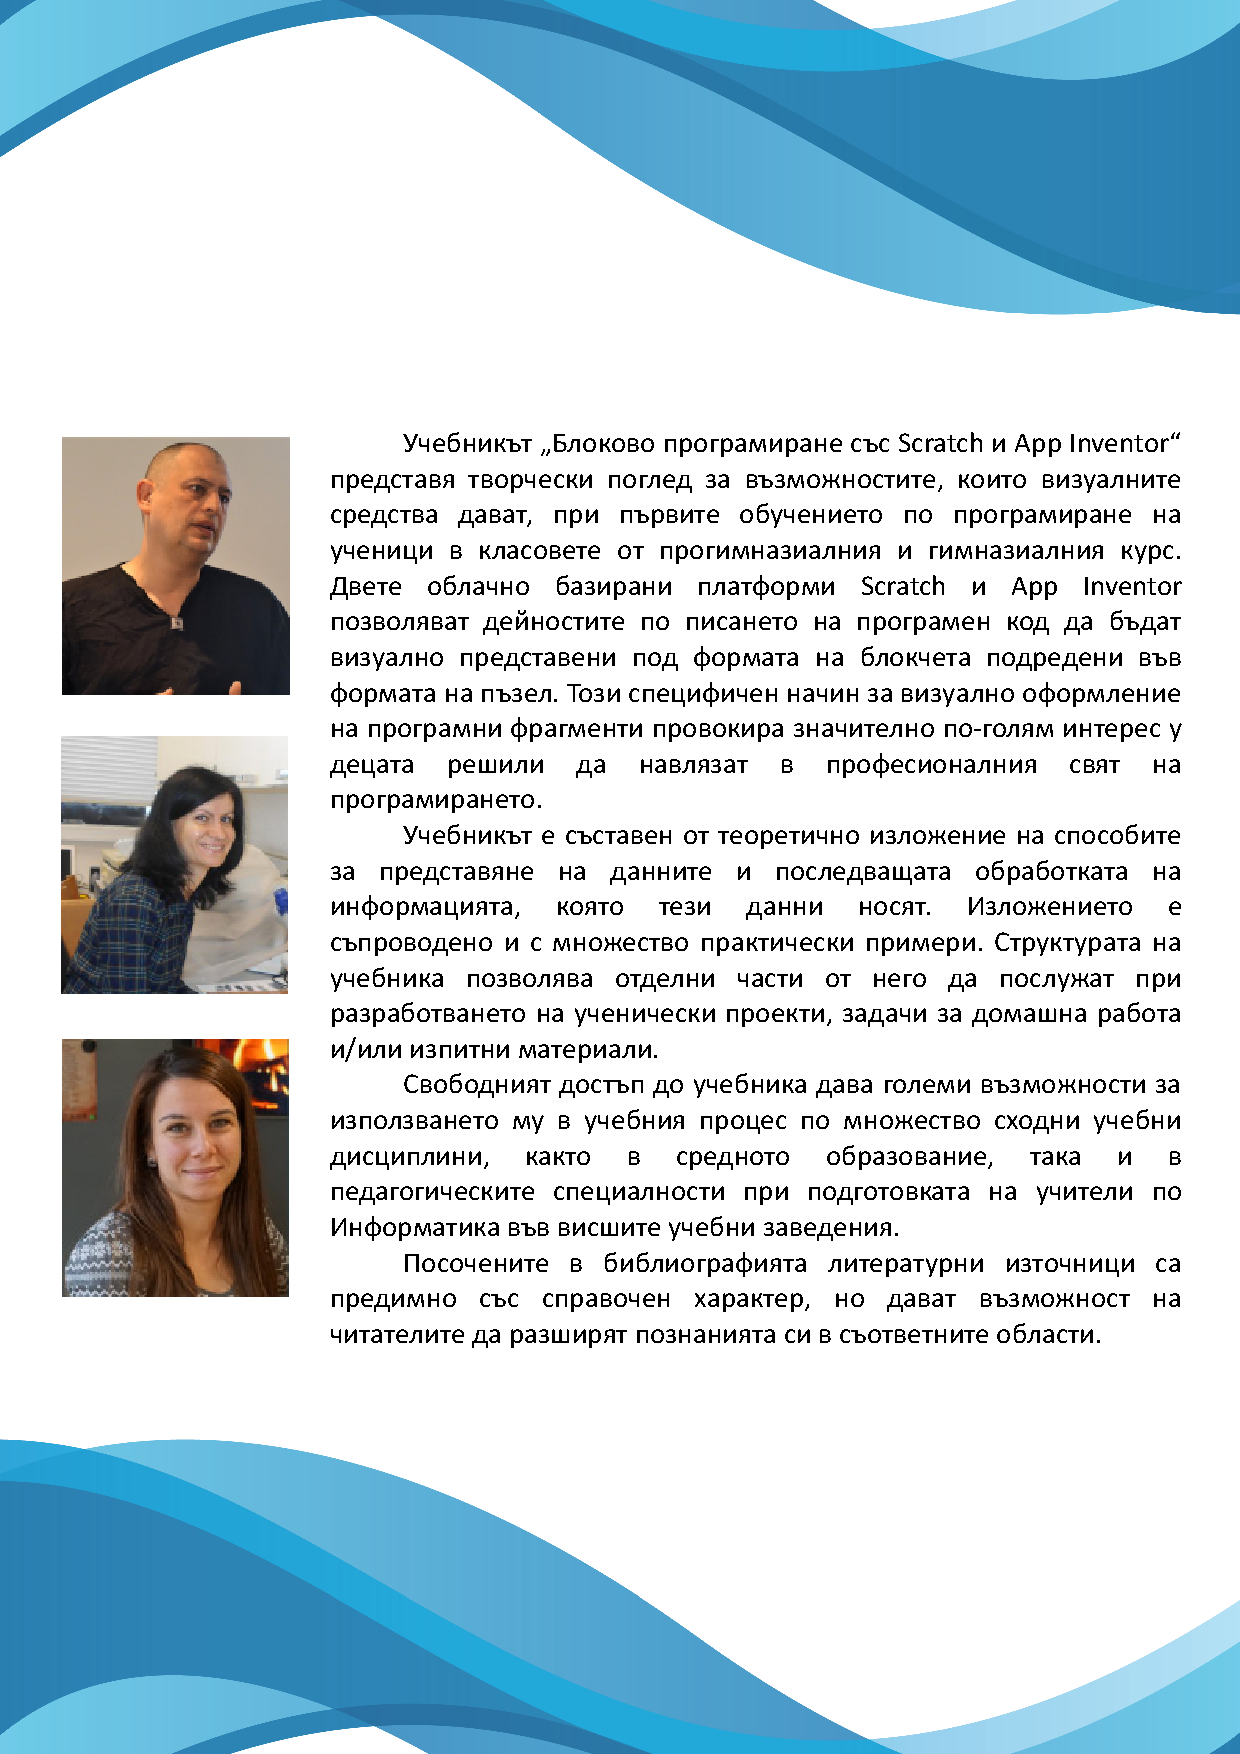
\includepdf[pages=-]{covers/back}

\end{document}
